\chapter{Fieldwork data analysis}
\label{Fieldwork_data_analysis}
Geological conditions are highly heterogeneous in northern Ghana. Subsurface characteristics vary at short mutual distances. Adequate and reliable information about local geohydrological conditions is preferably gathered through site-specific fieldwork. In this research perspective, multiple northern Ghana borehole locations are subjected to groundwater pumping tests. 
\bigskip \\
The NGO Conservation Alliance (CA) installed several PIT locations in the summer of 2016, in the Upper East and Northern Region. Pumping tests are performed at four of these boreholes. A fifth PIT borehole (in Ziong) is monitored to study how the ASR system is used by local farmers. The figure below shows a map  of the research locations in northern Ghana (Figure~\ref{fig:Overviewlocations}).
\bigskip 

\begin{figure}[ht]
 \centering
 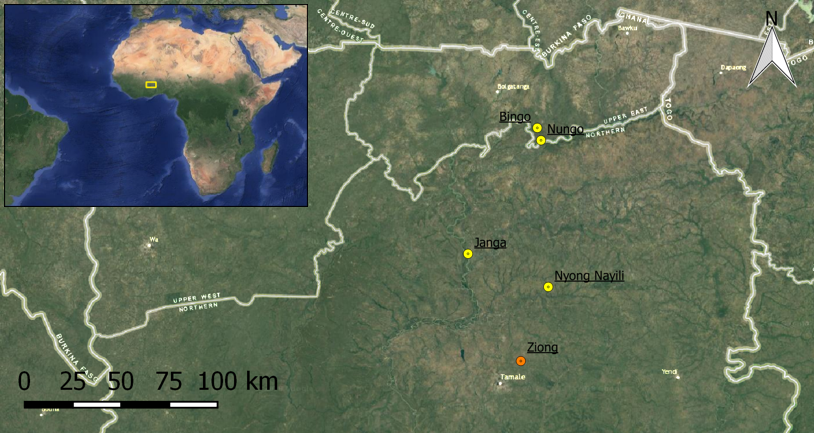
\includegraphics[width=\linewidth]{Overview_locations_northern_Ghana}
 \captionsetup{justification=centering} 
 \caption{Overview of fieldwork locations in northern Ghana}
 \label{fig:Overviewlocations}
\end{figure}

Detailed information on the equipment that was used, the set-up of the pumping tests as well as the monitoring of an operating ASR system can be found in appendix \ref{chapter:fieldwork_set-up}. The obtained raw fieldwork data can be found in the site-specific fact-sheets of appendix \ref{section:fieldworkresults}. The purpose of this fieldwork is to determine geohydrological subsurface parameters, transmissivity ($T$) and storativity ($S$), which are used as input for further investigation into upscaling these systems. 

This chapter contains the analysis of gathered fieldwork data. First, the methodology for data analysis, including some theoretical background, is explained (Section \ref{section:derivation_methods}). Section \ref{section:TS} contains the derivation of the local geohydrological parameter values: $T$ and $S$. Finally, the chapter concludes with the determination of parameter bandwidths (Section \ref{section:fieldwork_results}), which will be used in the subsequent model simulations. 

\section{Parameter derivation methods}
\label{section:derivation_methods}

\subsection{Theoretical model definition}
In large parts of northern Ghana the geohydrological soil characteristics are unknown. Strong variations at short mutual distance makes it necessary to obtain more information about local geology. The most reliable site-specific information was recorded during the drilling of boreholes (2016). The borehole log-sheets (appendix \ref{chapter:Borehole_logsheets}) are used as a starting point for the construction of the applied theoretical models in fieldwork analysis. 
\\

The site-specific borehole logsheets show similarities in stratification. In each case the upper 50 meters is divided into two or three layers, consisting of a confining top layer, and below that one or two "aquifers". Groundwater tables are predominantly positioned in the first aquifer. Based on these observations three simplified theoretical models for the analysis of fieldwork data are derived, as depicted in Figure \ref{fig:schematic_fieldwork_analysis}. 

\begin{figure}[h!]
	\centering
	\begin{subfigure}[b]{0.21\linewidth}
		\centering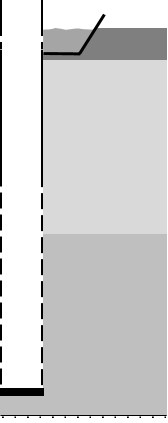
\includegraphics[width=0.6\linewidth]{Schematic_general_analysis}
		\captionsetup{justification=centering}		
		\caption{\label{fig:Schematic_general_analysis}}
		\end{subfigure}%\hfill
	\begin{subfigure}[b]{0.12\linewidth}
		\centering
\includegraphics[width=0.6\linewidth]{arrow_right}
		\end{subfigure}%\hfill
		%{\LARGE$\yrightarrow{}$}
	\begin{subfigure}[b]{0.21\linewidth}
		\centering
\includegraphics[width=0.6\linewidth]{Schematic_1lay_analysis}
		\captionsetup{justification=centering}		
		\caption{\label{fig:Schematic_1lay_analysis}}
		\end{subfigure}%\hfill
	\begin{subfigure}[b]{0.21\linewidth}
        \centering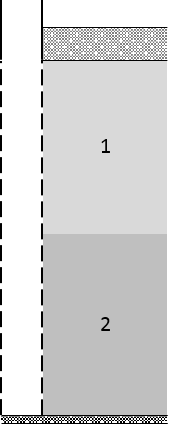
\includegraphics[width=0.6\linewidth]{Schematic_2lay_analysis}
		\captionsetup{justification=centering}		
		\caption{\label{fig:Schematic_2lay_analysis}}
		\end{subfigure}
	\begin{subfigure}[b]{0.21\linewidth}
        \centering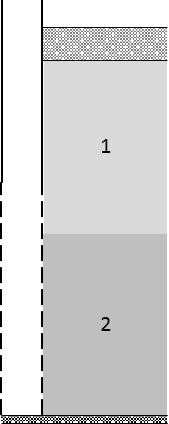
\includegraphics[width=0.6\linewidth]{Schematic_3lay_analysis}
		\captionsetup{justification=centering}		
		\caption{\label{fig:Schematic_3lay_analysis}}
		\end{subfigure}
	\captionsetup{justification=centering}	
	\caption{Schematic cross-sectional view of (\subref{fig:Schematic_general_analysis}) generalized northern Ghana soil stratification and simplified representations: (\subref{fig:Schematic_1lay_analysis}) a single layer system, ~(\subref{fig:Schematic_2lay_analysis}) a double layer system, and ~(\subref{fig:Schematic_3lay_analysis}) a system with two layers and partial penetration of the well} 
	\label{fig:schematic_fieldwork_analysis}
\end{figure} 

These simplified models (Figure \ref{fig:Schematic_1lay_analysis} - \ref{fig:Schematic_3lay_analysis}) mimic local conditions, making the derivation of representative hydraulic subsurface characteristics ($T$ and $S$) possible \citep{Kruseman2000}. Double layered models are applied to provide more degrees of freedom, potentially generating more accurate simulations. A maximum of two soil layers are implemented to limit chances of equifinality, due to an abundance of degrees of freedom. \\ 

\subsection{Techniques in analysis}
\label{section:techniques_analysis}
This section contains a description of the (analytical) models and methods used for optimal groundwater parameter estimation. \\


\textbf{Theis's method} \\ 
Groundwater drawdown due to the withdrawal of water can be determined analytically with Theis's equation (Equation \ref{eq:theis}). Theis's method is applicable on the situation depicted in \ref{fig:Schematic_1lay_analysis}; a constant rate pumping test in a fully penetrating well in a confined single layer aquifer \citep{Kruseman2000}. The analytical solution is suitable for obtaining a first indication of geohydrological parameters.   

\begin{equation}
\label{eq:theis}
 s = \frac{Q}{4\pi K D} exp1(u)
\end{equation}

\begin{equation}
 u = \frac{r^{2} S}{4 K D t}
\end{equation}

Where $s$ (m) is the drawdown at distance $r$ (m) from the well, $Q$ (m$^{3}$) is the constant well discharge , $KD$ (m$^{2}$/d) is the aquifer transmissivity ($KD$ = $T$), $S$ (-) is the aquifer storativity, $t$ (d) is the time measured from the start of pumping and $exp1$ is the exponential integral. The drawdown measurements in this research are limited to in-well measurements. The distance $r$ in Theis's equation is assumed to be the length of the well radius (0.0635 m). Theis's method is applicable for the time of pumping as well as the recovery process. The script below shows the implementation of Theis's method in Python.\\

\begin{python}[h!]
def drawdown(t, T, S):
    s = Qo / (4 * np.pi * T) * exp1(ro ** 2 * S / (4 * T *t))
    s[t > toff] -= Qo / (4 * np.pi * T) * exp1(ro ** 2 * S / (4 * T *(t[t>toff] - toff)))   
    return s
\end{python}

\textbf{Analytic Element Modelling in TTim}\\
TTim is a computer program based on analytic elements and designed for the analysis of transient groundwater flow in one or more layers. Multiple elements (and types of elements) can be added to specific predefined model layers. The use of TTim makes it possible to take additional well characteristics into account. Groundwater heads can be determined inside the well and the model optionally accounts for borehole storage and well skin resistance. Well discharge can be toggled on and off multiple times. This allows simulations of both single pumping and recovery tests and long-term well operations \citep{Mishra2013,Bakker2013}. \\

The analysis of the pumping and recovery tests is performed with the TTim \texttt{Model3D} configuration. The inclusion of a single well element is sufficient in this case. Depending on which subsurface model is used (Figure \ref{fig:schematic_fieldwork_analysis}) the well (analytic element) is screened in one or more model layers. The top layer is configured as phreatic layer, meaning the top layer storage coefficient ($S$) is a phreatic storage coefficient ($S_y$). This is based on observed initial groundwater tables, which are located below the bottom of the confining top layer. Multiplying this value with the aquifer thickness is therefore no longer needed. Each layer in the simplified model has a thickness of 1 meter. This means derived hydraulic conductivities ($k$) can be interpreted as transmissivities ($T$) and the storage is expressed as the layer storage coefficient ($S$). This is done to directly derive $T$ and $S$ values. Additionally, this approach automatically corrects for the unknown thickness of the deepest soil layer in which the well is screened. There is no information about soil conditions beyond the bottom of the wells in the borehole log-sheets (Appendix \ref{chapter:Borehole_logsheets}). \\

\textbf{MODFLOW}\\
The modelling of ASR upscaling scenario's (see Chapter \ref{chapter:model_scenarios}) is done with Modular Ground-Water Flow Model (MODFLOW), a finite difference model for groundwater flow developed by the U.S. Geological Survey (USGS). MODFLOW is the international standard in groundwater simulation (\citep{Niswonger2011,HarbaughArlen2005}). More information on the applied inputs can be found in Chapter \ref{chapter:model_scenarios}. In the case of fieldwork data analysis  MODFLOW is not used for the derivation of geohydrological parameters. Optimal parameters derived with TTim models are implemented in corresponding MODFLOW models to validate obtained TTim results.

\subsection{Optimization functions}
Pumping test data (section \ref{section:fieldwork_results}) is used as input for the derivation of local geohydrological parameter values. The values of $T$ and $S$ are determined by the method of (curve) fitting the analytical solutions and TTim models to the data. In this process two optimization functions are used. \\

\textbf{Fmin-RMSE optimization}\\
Differences between the measured and modelled drawdown curves can be expressed by the Root-Mean-Square-Error (Equation \ref{eq:RMSE}). The \texttt{Fmin} function (part of Python's \texttt{scipy.optimize} package) is applied to minimize the difference between modelled and observed drawdowns. This optimization results in optimal $T$ and $S$ values (and optionally values for borehole storage and well skin resistance) that represent local conditions. An example Python implementation of \texttt{Fmin} optimization is given below. It shows an optimization of five parameters ($T$ and $S$ values for two model layers and well skin resistance). \\ 

% example of monospace use: \texttt{hier wat je wilt hebben in monospace}!

\begin{equation}
\label{eq:RMSE}
 RMSE = \sqrt{\Sigma\frac{(s_{mod}-s_{field})^{2}}{N}}
\end{equation}

Where $s_{\text{mod}}$ is the modelled drawdown (m), $s_{\text{field}}$ is the observed drawdown (m) and N is the number of data points. \\
 
\begin{python}[h!]
def optimTTim_Qvar(params, t, meas):
    kaq = np.zeros(2)
    Saq = np.zeros(2)
    kaq[0] = params[0]             
    kaq[1] = params[1]
    Saq[0] = params[2]
    Saq[1] = params[3]
    res = params[4]
    s = drawdownTTim_Qvar(t, kaq, Saq, res)
    error = np.sqrt(np.mean((s-meas)**2)) 
    return error

xopt = fmin(optimTTim_Qvar, x0=[10, 10, .01, .001, 0.1], args=(to[mask], do[mask]), xtol=1e-4)
\end{python}
\bigskip

\textbf{Calibration function}\\
TTim has an in-built calibration function for the derivation of parameter values. Application of this second method improves the research robustness. In the Python script below, an example of the TTim \texttt{Calibrate} function is given. It is the same example as mentioned in the \texttt{Fmin} optimization above.\\ 

\begin{python}[h!]
cal = Calibrate(mlc)
cal.parameter(name='kaq0', layer=0, initial=10, pmin=0)
cal.parameter(name='kaq1', layer=1, initial=10, pmin=0)
cal.parameter(name='Saq0', layer=0, initial=.01, pmin=0, pmax=0.3)
cal.parameter(name='Saq1', layer=1, initial=.001, pmin=0, pmax=0.3)
cal.parameter(name='res', par=wc.res, initial=0.1)
cal.series(name='obs3', x=ro, y=0, layer=[0,1], t=to[mask], h=-do[mask])
cal.fit()
\end{python}

Both optimization methods require an initial estimate for the parameters. More than one suitable solution is possible, which makes the outcome of the optimization dependent on the choice of initial values. Other studies found that $T$ and $S$ values are commonly low in northern Ghana \citep[e.g.][]{Owusu2015,Owusu2017}. Based on these other studies the following initial conditions are applied: $k_{aq0}$ is 10 (m/d), $k_{aq1}$ is 10 (m/d), $S_{aq0}$ is 0.01 (-), $S_{aq1}$ is 0.001 (-) and well resistance is 0.1 (d). The actual well radius is used as the (initial) borehole storage: 0.0635 (m). Boundary conditions are applied to avoid the optimization resulting in physically improbable parameter values, i.e. negative parameter values and unnaturally high storativity values (greater than 0.3 (-)).

%(write something over initial conditions. Such small values. Not one single best solution. multiple 'best' solutions potentially close to each other. so solutions highly influential by the arbitrary chosen initial conditions. For each location several attempts done to see which initial conditions score pretty good. And subsequently generalization of those initial parameters applied per location/pumping test. for example better fit at Bingo at initial condition for T (KD) of 10, 10 (lay one and two) for fmin then for cal (2 layered system.) But 2 layered system all of sudden scores better with initial conditions 5, 1 for example.  

\section{From fieldwork data to $T$ \& $S$ values}
\label{section:TS}
The methods and models mentioned in the previous section are applied on the measurements from the five locations: Bingo, Nungo, Nyong Nayili, Janga and Ziong. Measurements results are included in the fact-sheets of Appendix \ref{section:fieldworkresults}. A complete overview of all optimization simulations (overall 25 per location) can be found in Appendix \ref{chapter:Extense_fieldwork_analysis}. Most important outcomes are discussed below for each of the five locations.

\subsection{Location: Bingo}

\textbf{Site inspection}\\
The surroundings of Bingo are characterized by a mildly sloping landscape. (Bed)rock appears occasionally at the surface. Site inspection showed an abundance of charred vegetation. The area is exposed to bush fires. As a consequence the agricultural field is not in operation. Map inspection shows the presence of the Volta river within several kilometres from Bingo. However, no indications of surface water (water-bodies and/or ponds) were observed. Bingo inhabitants label wet season flooding as high. Inundation levels of 1-2 m are common and usually last for several days. Flooding is not always caused by rain, every now and then a surplus of water accumulates at the surface by "popping up" out of ground. Inspection on the infiltration technology itself revealed the presence of a steel lid. Above surface level no well screen perforations were observed. The infiltration bed is an entrance path for the replenishment of groundwater.\\

\textbf{Measurement quality}\\
A malfunctioning power converter postponed the pumping test start. Since nightfall was a time limiting factor, the delay resulted in a shortened total test duration. In-well drawdown observation further downgraded the measurement quality. Well turbulence (due to pumping) caused the origin of a tangled rope. Hand measurements became more complicated and unreliable. An even more important consequence of the tangled rope was the occurrence of an undesirably high position of the deepest pressure sensor installed (see measurement set-up in Appendix \ref{section:measurement_structure}). Direct result is a long-term gap in pumping test drawdown data (yellow dotted line in Figure \ref{fig:Bingo_best}). The exact drawdown at the last moment of pumping is for example missing. Among other things due to the deliberate choice of a relative long-time recovery measurement the overall dataset can potentially be of use. \\

\textbf{Fit analysis} \\
The long-term absence of adequate data has its effects on the parameter fitting capabilities. As visible in Figure \ref{fig:Bingo_best}, Theis's method encounters difficulties here. Drawdown most definitely exceeded the measurement limit of 8m. This is not reflected in the parameter outcome of Theis's method. Defective fitting capabilities, due to a gab in data, are clearly less emphatically present in the analysis by the use of TTim.  Optimal parameter values are found at which drawdown curves exceed the drawdown measurement limit. Taking borehole storage and/or well resistance in consideration may potentially underlie this. This example shows it is not by definition required to feature complete drawdown data. By the use of TTim incomplete time series can result in adequate optimal parameter values. In order size the values found are low but align initial conditions. Furthermore it can be appointed that the double-layered transmissivity values found, suggest the presence of only one preferential layer of groundwater flow. \\

\begin{table}[h!]
\small
\centering
\caption{Bingo - overview best fit parameters}
\label{tab:bing_table}
\begin{tabular}{l|c|r|r|rr|rr|c}
\hline 
\textbf{}       & \textbf{Method} & \textbf{Stor [m]} & \textbf{Res [d]} & \textbf{T1}  & \textbf{T2   [m$^2$/d]}  & \textbf{S1}  & \textbf{S2 [-]}  & \textbf{RMSE [m]} \\ \hline \hline
Analytical                & fmin             & -             & -            & 10.83      & -          & 2.0e-04    & -          & 0.798 \\
1 lay                     & fmin             & 0.0647        & 5.6e-02      & 26.23      & -          & 6.6e-03    & -          & 0.163 \\
2 lay                     & fmin             & 0.0635        & -            & 2.8e-04    & 8.25      & 3.0e-03    & 2.1e-06    & 0.107 \\
2 lay (pp)                & fmin             & 0.0597        & -            & 8.6e-04    & 7.44      & 7.1e-03    & 6.3e-06    & 0.078 \\ \hline    
\end{tabular}
\end{table}

\begin{figure}[h!]
 \centering
 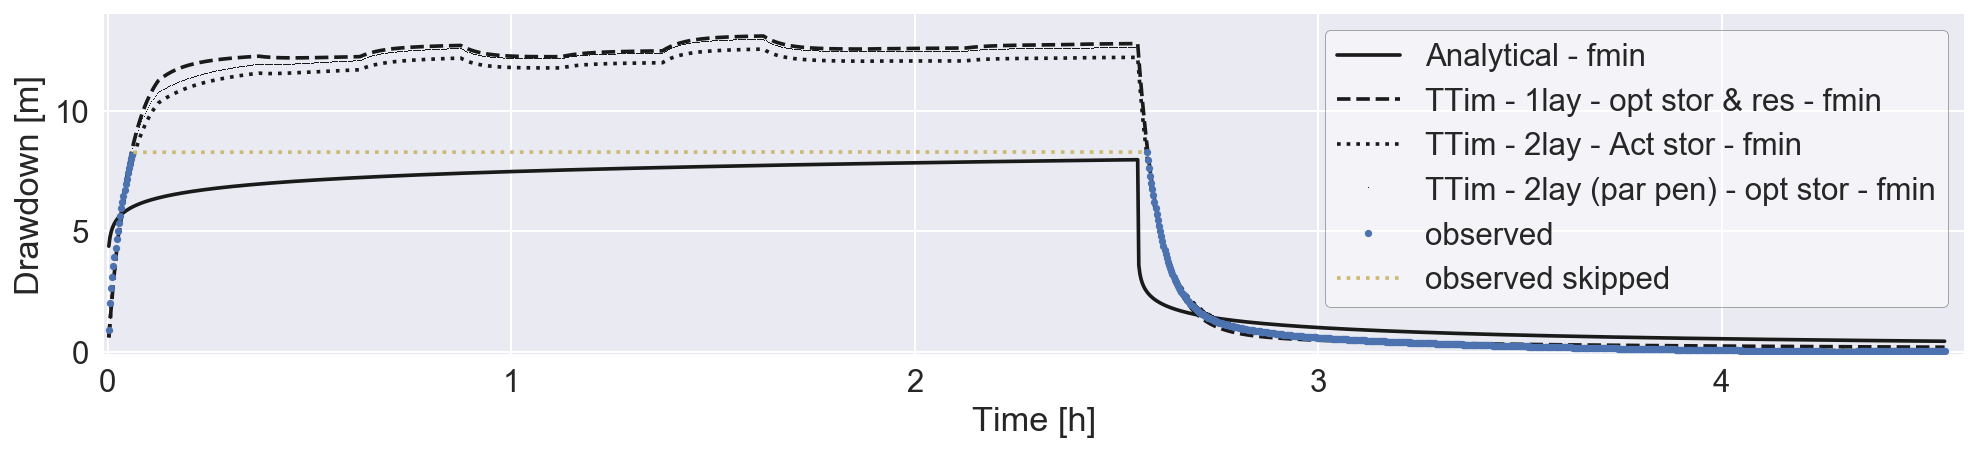
\includegraphics[width=\linewidth]{bingo_multi_lay_best}
 \captionsetup{justification=centering} 
 \caption{Bingo - Simplified models best fit}
 \label{fig:Bingo_best}
\end{figure}

\textbf{Substantive remark} \\
Both parameter optimization functions (\texttt{Fmin} and \texttt{Calibrate}) are able to derive reasonable solutions. Results of the \texttt{Calibrate}) optimization function reveal that an increase in model degrees of freedom not necessary leads to better performance (Appendix \ref{chapter:Extense_fieldwork_analysis}).Also by looking at the TTim best fit solutions (Figure \ref{fig:Bingo_best}) only minor distinction can be made in performance of the applied simplified models with a single layer, double layer or double layer with a partially penetrating well. Overall model accuracy slightly increases (Root-Mean-Square-Error slightly decreases) by an increase in complexity. An increase that can not be labelled as significant. All three simplistic theoretical models potentially represent nature properly by the in TTim found optimal parameters, depicted in Table \ref{tab:bing_table}.  

%\begin{figure}[h!]
%	\centering
%	\begin{subfigure}[b]{1\linewidth}
%		\centering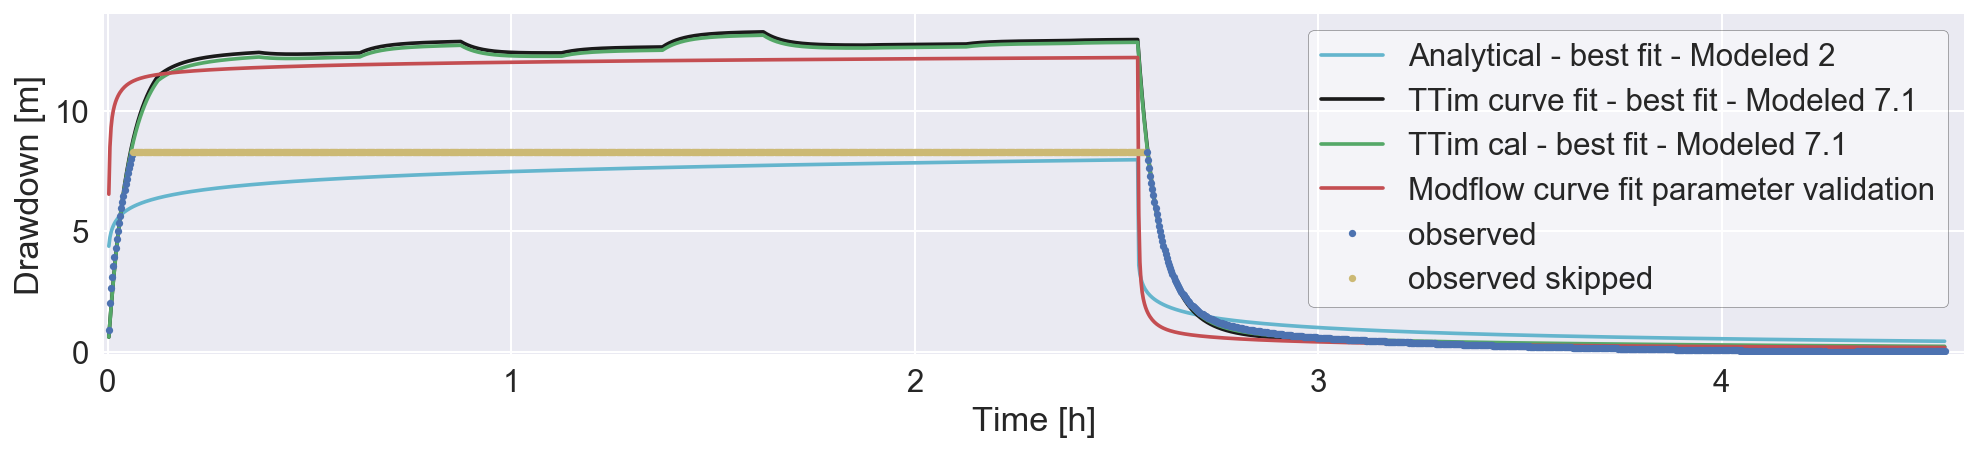
\includegraphics[width=1\linewidth]{bingo_1lay_analysis}
%		\captionsetup{justification=centering}		
%		\caption{\label{fig:bingo_1lay_analysis}}
%		\end{subfigure} \\ %\hfill
%	\begin{subfigure}[b]{1\linewidth}
%        \centering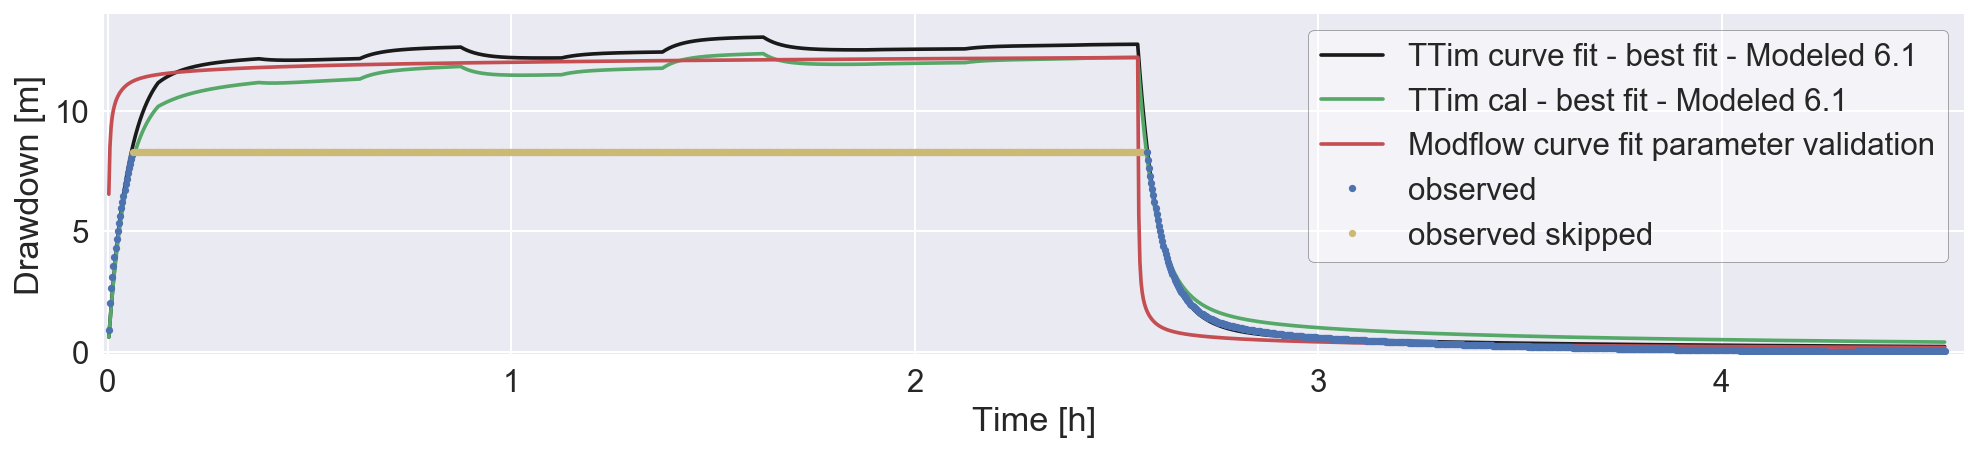
\includegraphics[width=1\linewidth]{bingo_2lay_analysis}
%		\captionsetup{justification=centering}		
%		\caption{\label{fig:bingo_2lay_analysis}}
%		\end{subfigure} \\
%	\begin{subfigure}[b]{1\linewidth}
%        \centering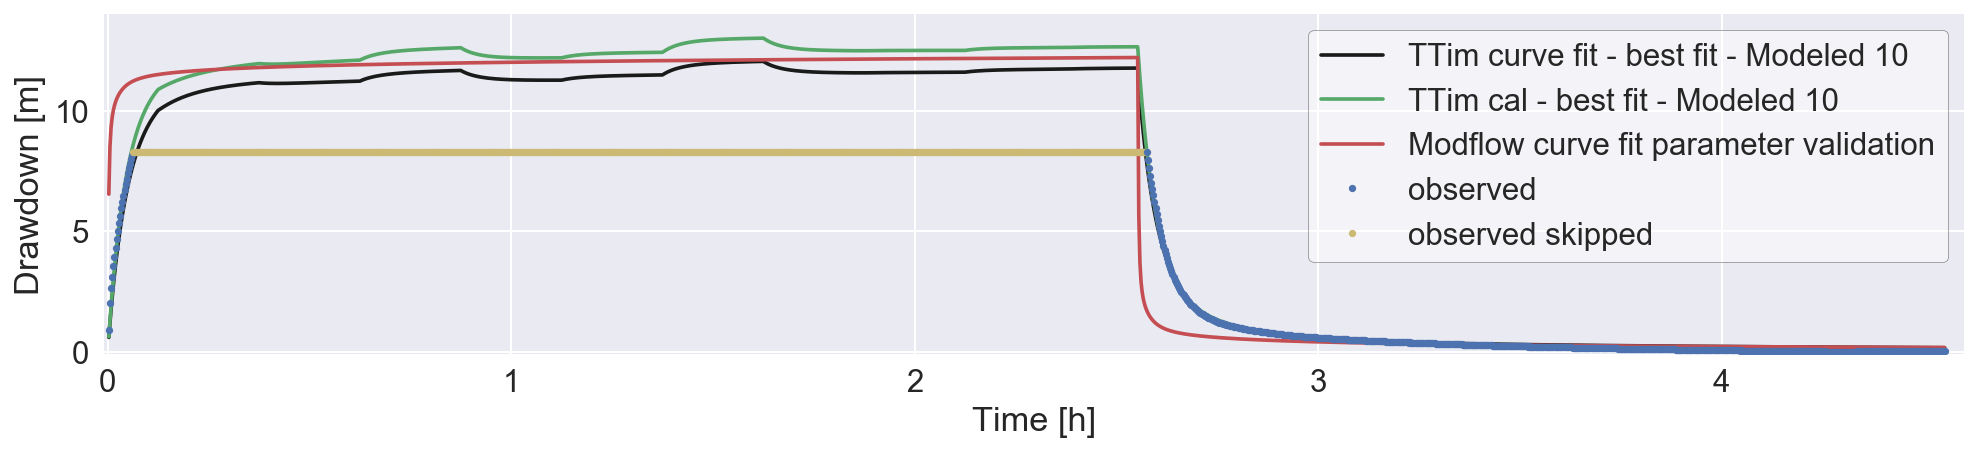
\includegraphics[width=1\linewidth]{bingo_3lay_analysis}
%		\captionsetup{justification=centering}		
%		\caption{\label{fig:bingo_3lay_analysis}}
%		\end{subfigure}
%	\captionsetup{justification=centering}	
%	\caption{Pumping test fit TS results: (\subref{fig:bingo_1lay_analysis}) single layered, ~(\subref{fig:bingo_2lay_analysis}) double layered and ~(\subref{fig:bingo_3lay_analysis}) triple layered (partially penetrating)} 
%	\label{fig:bingo_fieldwork_analysis}
%\end{figure} 

%
%\begin{table}[h!]
%\small
%\centering
%\caption{Bingo - overview best fit parameters}
%\label{tab:bingo_table}
%\begin{tabular}{l|l|l|lll|lll|l}
%\hline 
%\textbf{}       & \textbf{Stor [m]} & \textbf{Res [d]} & \textbf{T1}& \textbf{T2}  & \textbf{T3   [m$^2$/d]}  & \textbf{S1}& \textbf{S2}  & \textbf{S3 [-]}  & \textbf{RMSE [m]} \\ \hline
%\textbf{Single Lay}       & \textbf{} & \textbf{} & \textbf{}& \textbf{}& \textbf{}  & \textbf{}& \textbf{}& \textbf{}  & \textbf{}                    \\ \hline
%Analytical                & -             & -            & 10.83      & -          & -          & 2.0E-04    & -          & -          & 0.798         \\
%Curve fit                 & -             & 0.05         & 25.52      & -          & -          & 7.3E-05    & -          & -          & 0.166         \\
%Cal                       & -             & 2.5E-04      & 21.94      & -          & -          & 5.9E-19    & -          & -          & 0.175         \\
%{\textbf{}}               &               &              &            &            &            &            &            &            &               \\ 
%\textbf{Double Lay}       & \textbf{} & \textbf{} & \textbf{}& \textbf{}& \textbf{}  & \textbf{}& \textbf{}& \textbf{}  & \textbf{}                    \\ \hline
%Curve fit                 & -             & 0.06         & 22.88      & 0.40       & -          & 4.2E-04    & 8.0E-04    & -          & 0.167         \\
%Cal                       & -             & 0.02         & 11.63      & 0.57       & -          & 3.3E-07    & 4.7E-06    & -          & 0.413         \\ {\textbf{}}               &               &              &            &            &            &            &            &            &               \\ 
%\textbf{Triple Lay}       & \textbf{} & \textbf{} & \textbf{}& \textbf{}& \textbf{}& \textbf{}& \textbf{}& \textbf{}& \textbf{}                        \\ \hline
%Curve fit                 & -             & -            & 6.28       & 1.6E-03    & 0.86       & 1.8E-06    & 1.7E-02    & 2.0E-03    & 0.163         \\
%Cal                       & -             & -            & 17.95      & 3.76       & 3.35       & 0.18167    & 0.29988    & 0.11243    & 0.076         \\ \hline    
%\end{tabular}
%\end{table}

\subsection{Location: Nungo}

\textbf{Site inspection} \\
The remote community of Nungo is located in the Upper East region of Ghana. Access is possible by an unprepared road or river cross only. The landscape is mildly sloping till flat. Low afforestation is interspersed by plains. Adjacent to the community an out of use agricultural field is present. The Volta river looms a close range (approximately 400m). Wet season flooding occurs due to riverbank over-topping. Inhabitants label inundation levels as extreme. Water levels of 3m and higher persist for the entire rainy season. The groundwater infiltration technology is characterized by perforations above surface level. At the moment of inspection the top was distorted by heat. The closure by the use of a lid was thus excluded. \\
   
\textbf{Measurement quality} \\
Installation of the test set-up was heavily influenced by difficulties in pump immersion. From the first moment of pumping discharge rates were zero by approach. Well inspection revealed the presence of a liquid consisting of a combination of water, sandy clay and debris. The pumping test was restarted twice with a raised pump elevation. No improvements in outcomes were encountered. \\
  
\textbf{Fit analysis} \\
- \\

\textbf{Substantive remark} \\
Due to an aborted test no drawdown results perceived. The well is clogged and should be cleaned before measurements can be done.

\subsection{Location: Nyong Nayili}

\textbf{Site inspection} \\
The landscape of Nyong Nayili and her surroundings is typically flat. A mix of bushes, low vegetation and crop fields is present. During site inspection the agricultural field related to the infiltration technology of interest is not (yet) defined. The local community encounters wet season inundation levels up to 1 m. Within the season fluctuation occur, and can be explained by its rainfall based origin. During inspection no river or water flow is observed in the area. A muddy stagnant pond is present at close well range (approximately 40m). It definitely needs to be appointed, the infiltration bed is still inundated (approximately 0.2 m) during pumping test application. Well perforations reach above the infiltration bed. The accumulated water present definitely has its repercussions on the test. \\

\textbf{Measurement quality} \\
Start of the pumping test was delayed due to the well location search and the initial use of a clogged discharge hose. Since nightfall was a time limiting factor, the delay resulted in a shortened total test duration. In addition, the inundated infiltration bed heavily affected the pumping test. The first 20 minutes of drawdown measurements are labelled as useless due to an (unknown) additional inflow (see Appendix \ref{section:fieldworkresults}). This period is not taken into account during further analysis. Visual inspection during pumping test application implies the interference of additional inflow even beyond this 20 minutes data skip. Usability of the data set (especially during pumping) can therefore be questioned. \\
 
\textbf{Fit analysis} \\
Theis's method encounters difficulties in finding adequate parameter values. The optimal solution does not result in a reasonable curve fit (compared to data-set). Found storativity equals the predefined upper bound. The solution is unreliable and can be neglected. The use of TTim has a positive impact on the outcome in data analysis. Found transmissivity values are not analogous, but potentially represent nature. Storativity values can be interpreted as low. Obtained optimal borehole storage values are strikingly high. These values potentially reflect the presence of additional inflow. Being a constant value, this reflection only accounts to a certain extent. Overall curve fitting performances are moderate. The lack in fitting capabilities can potentially be attributed to the data skip and/or the unknown additional inflow of water over time. \\

\begin{table}[h!]
\small
\centering
\caption{Nyong Nayili - overview best fit parameters}
\label{tab:Nyong_Nayili_table}
\begin{tabular}{l|c|r|r|rr|rr|c}
\hline 
\textbf{}       & \textbf{Method} & \textbf{Stor [m]} & \textbf{Res [d]} & \textbf{T1}  & \textbf{T2   [m$^2$/d]}  & \textbf{S1}  & \textbf{S2 [-]}  & \textbf{RMSE [m]} \\ \hline \hline
Analytical                & fmin             & -             & -            & 6.00       & -          & 3.0e-01    & -          & 0.752 \\
1 lay                     & cal              & 0.2419        & -            & 13.35      & -          & 7.8e-05    & -          & 0.457 \\
2 lay                     & cal              & 0.2436        & -            & 6.95       & 6.98       & 4.6e-06    & 3.6e-05    & 0.457 \\
2 lay (pp)                & fmin             & 0.2659        & 1.7e-02      & 1.7e-04    & 28.61      & 1.1e-02    & 4.4e-06    & 0.450 \\ \hline    
\end{tabular}
\end{table}

\begin{figure}[h!]
 \centering
 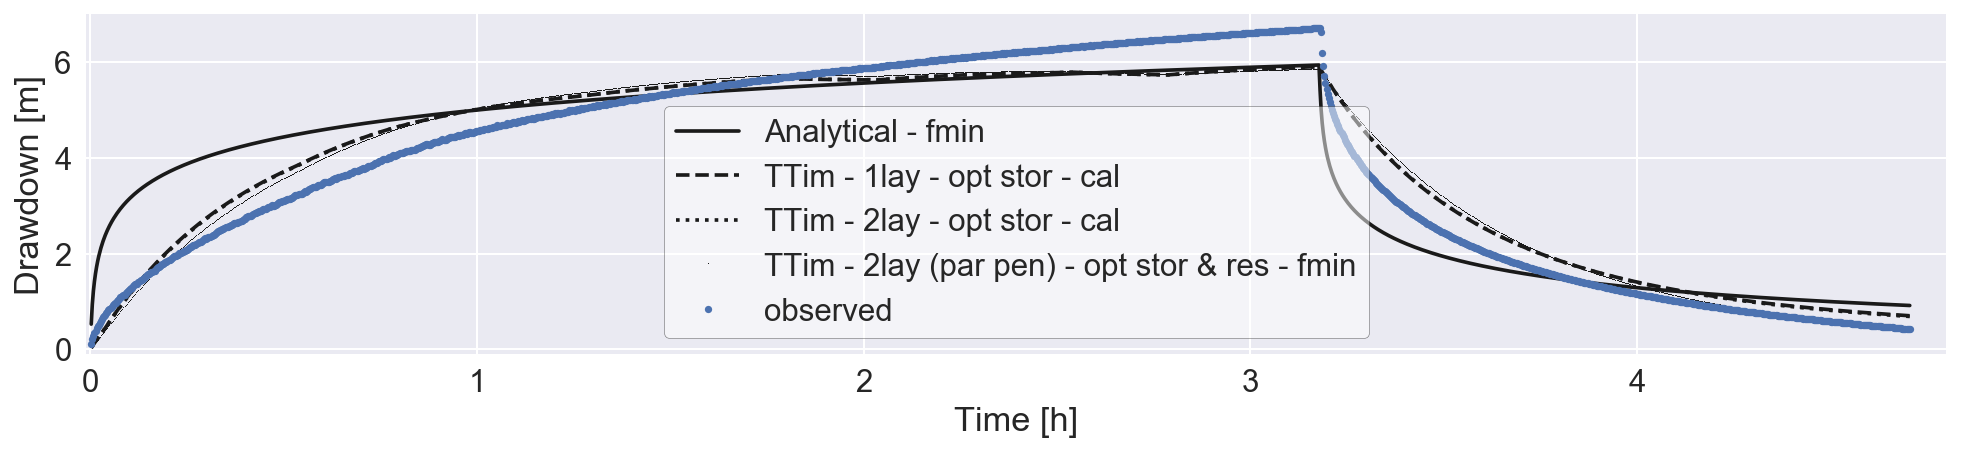
\includegraphics[width=\linewidth]{Nyong_Nayili_multi_lay_best}
 \captionsetup{justification=centering} 
 \caption{Nyong Nayili - Simplified models best fit}
 \label{fig:Nyong_Nayili_best}
\end{figure}

\textbf{Substantive remark} \\
Deviations in obtained data-set and the different (TTim) modelled optimal simulations are of equal size, regardless the optimization function applied. An increase in parameter freedom does not necessarily improve model performance. Reverse effects do occur. In all model simulations the Root-Mean-Square-Error is substantial. The accuracy of the found optimal parameter values can therefore be doubted. Further research on the impact of missing starting data and/or the impact of water inflow during a pumping test is advised.  

\subsection{Location: Janga (1/2)}

\textbf{Site inspection} \\
The infiltration technology near Janga is potentially located at the bank (edge) of a dry river bed. The Volta river is located at walking distance (see fact-sheet visualisation, Appendix \ref{section:fieldworkresults}). A stagnant pond is present at a distance of approximately 70 m from the well. Wet season flooding is caused by river overflow. The flooding is labelled as constant, extreme (>4m) and lasts for months. During field visit no agricultural field is encountered related to the infiltration technology. The pipe segment above surface level accommodates perforations and is equipped with a plastic/concrete cover. \\ 

\textbf{Measurement quality} \\
Bush fires are abundant in the region. Due to close range appearance the test is aborted just before sunset. The duration of recovery process monitoring is affected. Noteworthy is the color change in water discharged during the pumping test. Alternately the water switched color (brownish, grey, white, clear) several times. No further complications occurred. The gathered data can potentially be of use for analysis. \\

\textbf{Fit analysis} \\
Found parameter order size is in line with the data gathered at the other research locations. This does not apply for the Root-Mean-Square-Error scale size. Large RMSE-values can be attributed to the pumping test drawdown part. Shape of the time series is most definitely worth-mentioning. Regardless which method and/or model applied, not a single combination is capable of approaching the remarkable drawdown shape. Analytical Theis method as well as TTim is not capable of correction for irregular patterns of groundwater tables over time. \\

\begin{table}[h!]
\small
\centering
\caption{Janga first attempt - overview best fit parameters}
\label{tab:Janga1_table}
\begin{tabular}{l|c|r|r|rr|rr|c}
\hline 
\textbf{}       & \textbf{Method} & \textbf{Stor [m]} & \textbf{Res [d]} & \textbf{T1}  & \textbf{T2   [m$^2$/d]}  & \textbf{S1}  & \textbf{S2 [-]}  & \textbf{RMSE [m]} \\ \hline \hline
Analytical                & fmin             & -             & -            & 8.84       & -          & 3.0e-01    & -          & 1.339 \\
1 lay                     & fmin             & 0.0635        & -9.7e-03     & 9.09       & -          & 1.6e-02    & -          & 1.382 \\
2 lay                     & fmin             & 0.1287        & -            & 12.48      & 1.3e-04    & 1.9e-02    & 1.1e-08    & 1.445 \\
2 lay (pp)                & fmin             & 0.0635        & -            & 9.1e-05    & 15.19      & 4.3e-08    & 3.1e-03    & 1.530 \\ \hline    
\end{tabular}
\end{table}

\begin{figure}[h!]
 \centering
 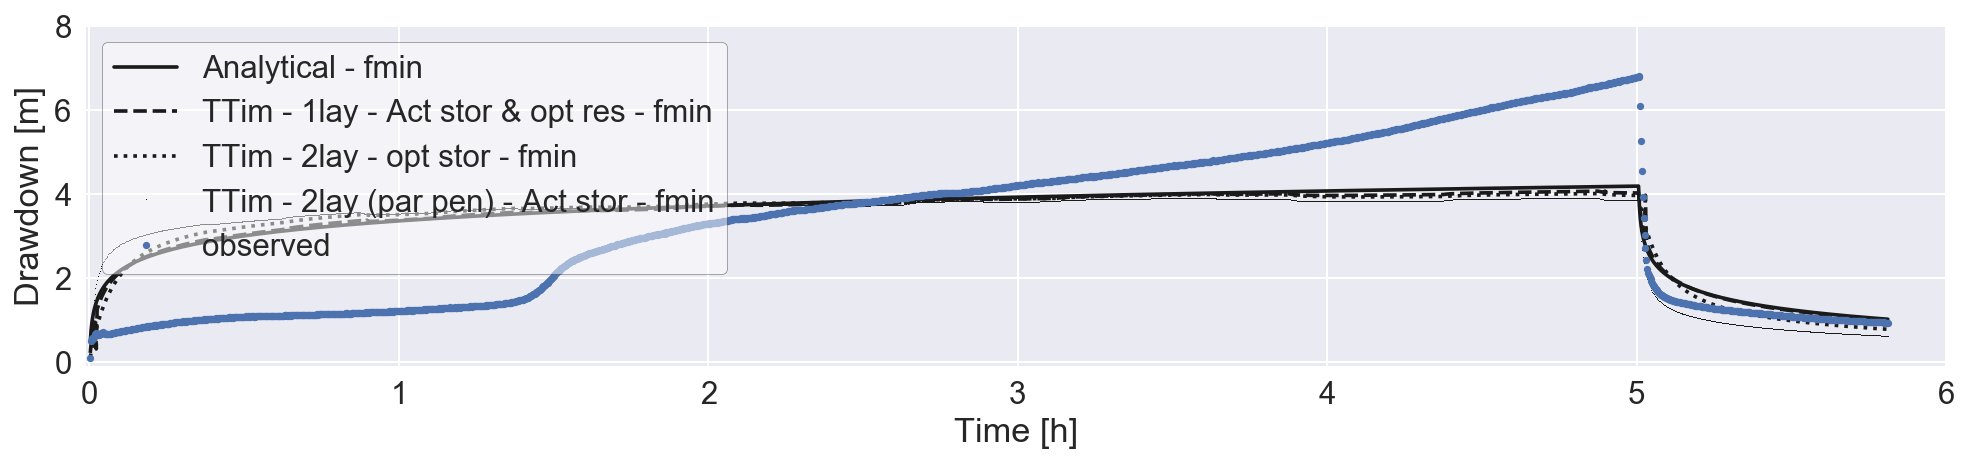
\includegraphics[width=\linewidth]{Janga1_multi_lay_best}
 \captionsetup{justification=centering} 
 \caption{Janga first attempt - Simplified models best fit}
 \label{fig:Janga1_best}
\end{figure}

\textbf{Substantive remark} \\
The course of the drawdown curve is most definitely catching the eye. Several details are striking. There is a sudden increase in drawdown after 90 minutes of pumping. Towards the end of pumping period (four to five hours) the curve does not show the characteristic behaviour of movement towards a new equilibrium. And the fluctuations are no longer monitored in the recovery process. As stated by \citet{Kruseman2000}, most of the time there is not a unique theoretical solution for these well-flow problem. Making the identification of the right (theoretical) system more difficult. Additional fieldwork can provide solutions. Validation is applied to confirm or disprove the correctness of the data-set. The same ASR system is exposed to a second pumping test.

\subsection{Location: Janga (2/2)}

\textbf{Measurement quality} \\
Initial (first two hours) pumping test discharge rates vary slightly (Appendix \ref{section:fieldworkresults}). The drawdown curve is potentially affected. Just as in the first attempt, the extracted water changed color several times. Compared to the previous research a longer monitoring of the recovery process is applied. The collected pumping test time series data is presumably useful. \\

\textbf{Fit analysis} \\
Despite the application of a lower rate pumping test (compared to first attempt) the  gathered drawdown data shows similar behaviour. Lower values in Root-Mean-Square-Error can be assigned to the lower general drawdown pursued and the increased duration of recovery monitoring. It does not necessarily mean the obtained parameter values are more reliable. Values as depicted in Table \ref{tab:Janga2_table} are at most useful as a plausible indication. 

\begin{table}[h!]
\small
\centering
\caption{Janga second attempt - overview best fit parameters}
\label{tab:Janga2_table}
\begin{tabular}{l|c|r|r|rr|rr|c}
\hline 
\textbf{}       & \textbf{Method} & \textbf{Stor [m]} & \textbf{Res [d]} & \textbf{T1}  & \textbf{T2   [m$^2$/d]}  & \textbf{S1}  & \textbf{S2 [-]}  & \textbf{RMSE [m]} \\ \hline \hline
Analytical                & fmin             & -             & -            & 15.97      & -          & 3.0e-01    & -          & 0.571 \\
1 lay                     & fmin             & 5.4e-07       & -9.7e-03     & 13.54      & -          & 1.9e-02    & -          & 0.551 \\
2 lay                     & fmin             & 0.2228        & -2.2e-02     & 2.05       & 8.13       & 2.1e-02    & 4.1e-04    & 0.545 \\
2 lay (pp)                & fmin             & 0.2005        & -3.1e-02     & 6.59       & 0.86       & 9.4e-05    & 2.1e-03    & 0.545 \\ \hline    
\end{tabular}
\end{table}

\begin{figure}[h!]
 \centering
 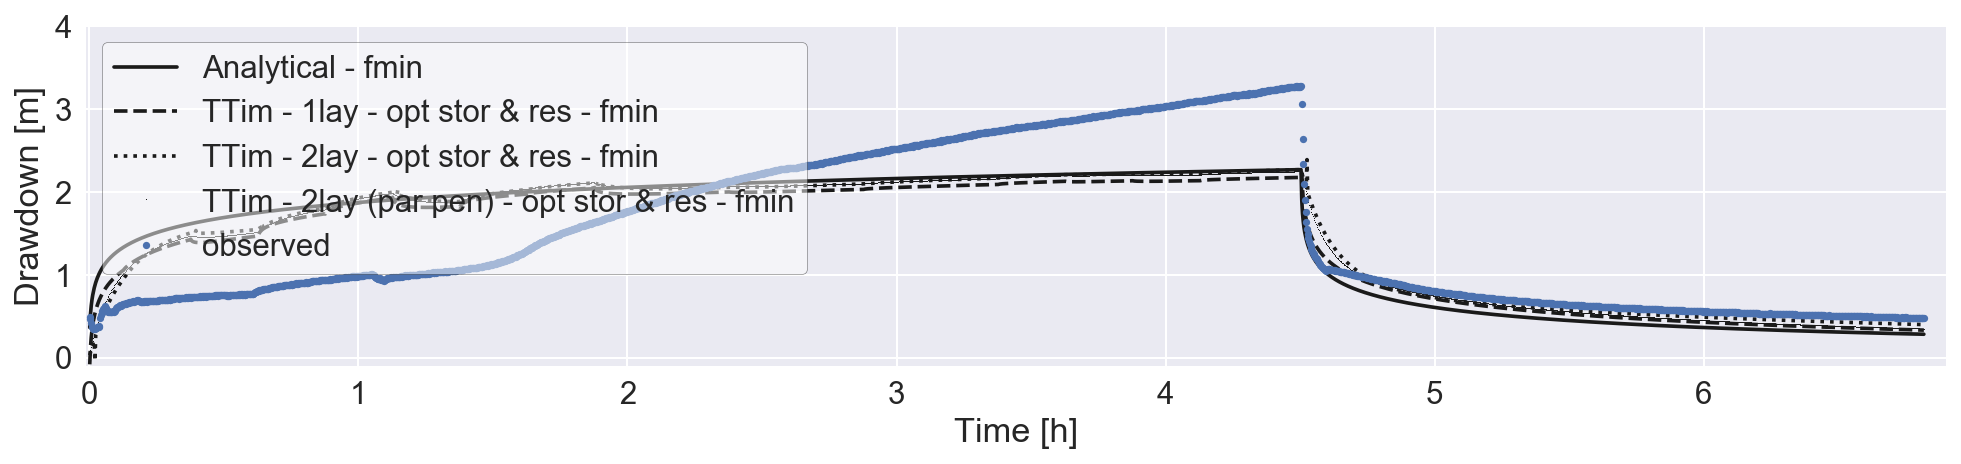
\includegraphics[width=\linewidth]{Janga2_multi_lay_best}
 \captionsetup{justification=centering} 
 \caption{Janga second attempt - Simplified models best fit}
 \label{fig:Janga2_best}
\end{figure}

\textbf{Substantive remark} \\
The applied validation confirms the correctiveness in data gathering. Nevertheless the uncertainty in theoretical model selection persist. A conclusion confirmed by \citet{Kruseman2000}. Causes of the authentic drawdown curve can be widespread. One can think of the drying preferential flow-path  layers, distinctive subsurface connections to the river bed, fracture zones and more. Instead of further fieldwork investigation, it is advisable to gain knowledge in complex drawdwon data interpretation. 

\subsection{Location: Ziong (monitoring)}

\textbf{Site inspection} \\
In the local surroundings of Ziong no river, water flow or ponds are perceived. Wet season land inundation is typically less than 2 m. Day to day variations takes place due to its origin by temporal heavy rain. The regional landscape is flat. Occasionally (bed)rock is observed at the surface. High grasses and bushes are present. Nature is supplemented by several agricultural fields. The infiltration technology does not contain tube perforations above surface level. A steel lid is present to cover the top inlet. Inspection showed the agricultural field related to the ASR-system is ready for the supply of water. \\

\textbf{Measurement quality} \\
During inspection the system was put in daily operation. Instead of a single pumping test, an unique opportunity is seized by an improvised monitoring of the system performance over multiple days. Due to the permanent seasonal pump installation and the limits of diver memory, monitoring divers are positioned in the borehole by an hanging rope only. The inescapable high positioning of the divers (above lowest encountered groundwater tables) results in the absence of multiple time-series segments (yellow dotted line in \ref{fig:Ziong_best}). The adopted discharge rate of 20 m$^3$/d is based on multiple time measurements of the present dated volume meter. In analysis it is assumed to be constant. Operational hours of pumping are not precisely known. In data analysis it is assumed recovery starts four minutes before the first sign of recovery appears in data. Despite these defects the collected data can be used for further analysis. \\

\textbf{Fit analysis} \\
Given the measurements nature no parameter definition is applied by the use of the analytical Theis method. Analysis by the use of TTim show reasonable results. Curve fit simulation shows thorough overlap with the measured time-series. This example shows the wide deployment of TTim. Although above areal prevailing, storativity values are plausible. Obtained transmissivity values are extremely low, but generally consistent. \\

\begin{table}[h!]
\small
\centering
\caption{Ziong - overview best fit parameters}
\label{tab:Ziong_table}
\begin{tabular}{l|c|r|r|rr|rr|c}
\hline 
\textbf{}       & \textbf{Method} & \textbf{Stor [m]} & \textbf{Res [d]} & \textbf{T1}  & \textbf{T2   [m$^2$/d]}  & \textbf{S1}  & \textbf{S2 [-]}  & \textbf{RMSE [m]} \\ \hline \hline
1 lay                     & fmin             & 0.0382        & -            & 1.76      & -         & 1.1e-03    & -          & 0.255 \\
2 lay                     & fmin             & 0.0635        & -0.05        & 0.38      & 1.05      & 2.9e-02    & 1.2e-03    & 0.240 \\
2 lay (pp)                & fmin             & 0.0147        & -0.08        & 0.23      & 0.78      & 2.6e-02    & 1.3e-03    & 0.243 \\ \hline    
\end{tabular}
\end{table}

\begin{figure}[h!]
 \centering
 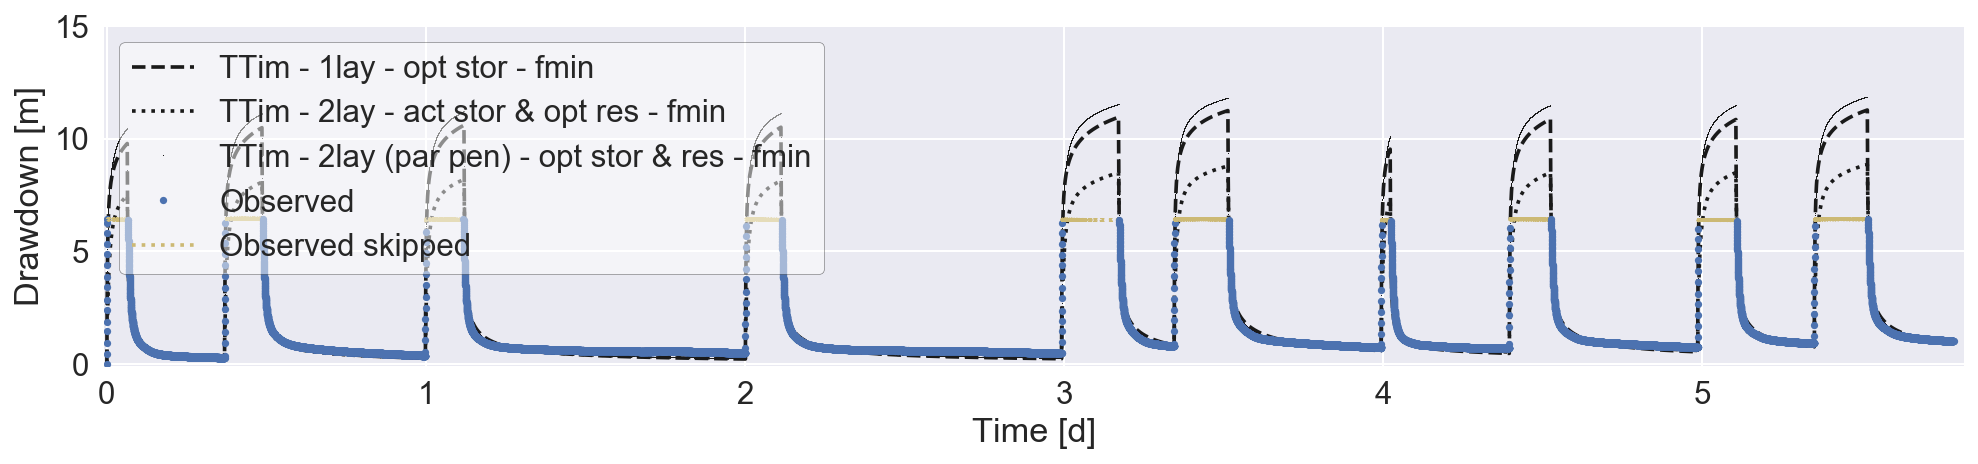
\includegraphics[width=\linewidth]{Ziong_multi_lay_best}
 \captionsetup{justification=centering} 
 \caption{Ziong - Simplified models best fit}
 \label{fig:Ziong_best}
\end{figure}

\textbf{Substantive remark} \\
Both optimization functions (\texttt{Fmin} and \texttt{Calibrate}) can be used for the generation of reasonable parameter outcome. When applying a simplified model with an increased number of degrees of freedom, the \texttt{Fmin} optimization function tends to score slightly better on values for the Root-Mean-Square-Error (Appendix \ref{chapter:Extense_fieldwork_analysis}). This however concerns a single measurement analysis, with a single set of predefined initial parameter. Moreover no other objective functions are taken into account. Regarding the optimisation functions no additional conclusions can be drawn. Looking at the performance of the different simplified models no line of improvement is discovered. Models with an  increased number of degrees of freedom do not necessarily represent nature better. Sometimes reverse effects are even effective. By the use of the right optimal parameter set all three simplified theoretical models are capable to represent the local nature of Ziong to a certain extend. 


%\section{Theoretical validation}
%
%\textbf{Soil analysis}
%
%\textbf{VES analysis}


\section{Results \& conclusions}
\label{section:fieldwork_conclusions}
A brief elaboration on key findings regarding the applied fieldwork pumping tests and data analysis is stated below. The section concludes with parameters definition, applicable on subsequent research. \\

\textbf{ASR-system performance}
\begin{itemize}
\item ASR-system cleaning \\
The ASR-systems of interest are exposed to natural forces. Only one year after construction (2016) the penetration depth of all five boreholes has shrunk. The order of impact differs per location. Most striking example is the borehole at location Nungo. Be aware of the relative fast system degradation. Measures should be taken to prevent the occurrence of clogging. It is advisable to provide each borehole with a plastic/concrete lid. Tube penetrations above the infiltration bed should be sealed permanently to avoid inflow of undesired particles. In addition, annual based preventive cleaning of borehole and infiltration bed is desirable.
         
\item Complementary research \\
Obtained pumping test drawdown data is potentially plausible. Nevertheless, uncertainty in the derivation of parameters and the selection of a (simplified) model consists. As stated by \citet{Kruseman2000}, additional fieldwork does not necessarily solve these uncertainties. No new comparable pumping tests at the same borehole locations are needed at short term. Gaining knowledge on the interpretation of data can possibly offer solutions. Complementary research on how to deal with gabs in pumping test data and/or irregularities in drawdown time-series is advisable. Moreover, future research can be pointed at the impact of (time-dependent) inflow of water during pumping test application. 

\item Future test applications \\
If applied, additional pumping tests should be targeted at the impact of ASR-systems on its surroundings. Pumping tests should be applied in combination with at least one (preferably more) piëzometer at a certain known distance from the well \citep{Kruseman2000}. These tests potentially generate insight in well skin behaviour (degree of resistance). \
The year round installation of one or more divers is an option if complete ASR-system understanding is desirable. This can provides more accurate or new system interpretations. To succeed, it is advisable to set up a measurement plan in advance. Generated data can be used for a more optimal system use.  
\end{itemize}

\textbf{Applicability of methods \& models}
\begin{itemize}
\item Functionality (analytical) methods; Theis \& TTim \\
Compared to the conventional pumping test Theis's method, TTim offers many more model options (borehole storage, well skin resistance, multiple layers) in drawdown data analysis \citep{Mishra2013,Bakker2013}. In this research TTim unsurprisingly outperforms Theis's method. Yet, the attendance of irregular drawdown time-series shows that TTim (e.g. analytical element modelling) also encounters limitations. 

\item Functionality optimization functions; \texttt{Fmin} \& \texttt{Calibrate} \\
Obtained geohyrological parameters represent local nature to a certain extend. This is confirmed by the Root-Mean-Square-Error values (objective function). Application of the two optimization functions generates outcomes. The results of corresponding optimizations can differ in parameter size, but accuracies (RMSE) are comparable (some exceptions). It can be concluded that both optimization functions (\texttt{Fmin} and \texttt{Calibrate}) are potentially usable for the determination of suitable $T$ and $S$ values. 

\item Functionality simplified models  \\
Representation of local nature is pursued by the use of three simplistic system: a single layer system, a double layer system and a system with two layers and partial penetration of the well (Figure \ref{fig:Schematic_1lay_analysis} - \ref{fig:Schematic_3lay_analysis}). Based on the Root-Mean-Square-Error objective function none of these systems sticks out positively or negatively. Therefore, subsequent parts of this research are carried out by the use of the (most simplistic) single layer system. This puts the emphasis on the main goal of this research; effects of ASR-system upscaling.  
\end{itemize}

\textbf{$T$ \& $S$ value definition} \\
Drawdown measurements are performed within the extraction well. A set-up which deviates from the desired common standard \citep{Kruseman2000}. It should be kept in mind the correctness of data can be questioned. From the perspective of robustness two optimization functions (\texttt{Fmin} \& \texttt{Calibrate}) are applied in data analysis. Comparative system optimizations obtain parameters of different size, while Root-Mean-Square-Error values are similar (some exceptions). Moreover, local nature can be represented equally good by a diversity of (single and/or double layered) simplistic systems. For each individual location there is more than one representative parameter-set available. In short, by the analysis of fieldwork data an abundance of uncertainties in parameter definition are present. \\

A bandwidth is defined to deal with these uncertainties. Upper and lower $T$ and $S$ values are stated around the single layer "best" fit solution (Bingo). A visualization of the bandwidth can be found in Figure \ref{fig:Parameter_bandwidth}.   Transmissivity extremes are based on the combination of obtained values in data analysis and a factor of safety. Definition of the outer storativity values needed a different approach. Found values in data analysis more than once approached the predefined boundaries conditions (0 and 0.3 (-)) (Appendix \ref{chapter:Extense_fieldwork_analysis}). These physically improbable parameters are ignored. Outer parameters are preferably based on more common applied values. The chosen lower limit storativity ($S_lower$) corresponds with the situation of a confined aquifer, while the upper limit ($S_upper$) is more related to the specific yield of a phreatic storage (bron: geo1) \citep{Strack1989,Fitts2012}. \\

\begin{figure}[h!]
 \centering
 
\includegraphics[width=0.6\linewidth]{Parameter_bandwidth}
 \captionsetup{justification=centering} 
 \caption{$T$ \& $S$ bandwidth selection}
 \label{fig:Parameter_bandwidth}
\end{figure}

The defined scope can not be interpreted as a generalization of the different locations. Not a single combination of the upper and lower parameter boundaries is the one on one representation of a specific location. The bandwidth predominantly acts as an input for scenario modelling in the subsequent parts of this research. Outcome of these scenarios can only be interpreted as indication of the ASR-system possibilities within northern Ghana. 